\subsection{不等式}\label{sec:4.7}
\autoref{sec:3.6} 介绍了用概率论证导出的不等式. 本节介绍的不等式适用于概率和期望，但论证基于函数与数的性质.
\subsubsection{数值不等式}\label{sec:4.7.1}
本小节的不等式虽然常以期望的形式表述，却主要依赖数的性质. 事实上，它们都基于下面这个简单引理.
\begin{lemma}\label{lem:4.7.1}
设 $a,b$ 为任意正数，$p,q$ 为满足
\begin{equation}\label{eq:4.7.1}
\frac1p+\frac1q=1
\end{equation}
的任意正数（因而必大于 1）. 则
\begin{equation}\label{eq:4.7.2}
\frac1pa^p+\frac1qb^q\ge ab,
\end{equation}
等号成立当且仅当 $a^p=b^q$.
\end{lemma}
\sourcepageanchor{184}

\begin{proof}
固定 $b$，考虑函数
$$g(a)=\frac1pa^p+\frac1qb^q-ab.$$
为求其最小值，求导并令导数为 0：
$$\frac d{da}g(a)=0\quad\Longrightarrow\quad a^{p-1}-b=0\quad\Longrightarrow\quad b=a^{p-1}.$$
检查二阶导数可知，这的确是极小值. 此时函数值为
$$\begin{aligned}
\frac1pa^p+\frac1q(a^{p-1})^q-aa^{p-1}
&=\frac1pa^p+\frac1qa^p-a^p&&\text{（由\eqref{eq:4.7.1}，$(p-1)q=p$）}\\
&=0.&&\text{（再次利用\eqref{eq:4.7.1}）}
\end{aligned}$$
所以最小值为 0，\eqref{eq:4.7.2} 得证. 最小值点唯一（为什么？），因此等号仅当 $a^{p-1}=b$ 时成立；由\eqref{eq:4.7.1}，这又等价于 $a^p=b^q$.
\end{proof}
第一个期望不等式是最常用、最重要的不等式之一，由此引理很容易得到.
\begin{theorem}[H\"older 不等式]\label{thm:4.7.2}\index{SI0568@Hölder}
设 $X,Y$ 为任意两个随机变量，$p,q$ 满足\eqref{eq:4.7.1}. 则
\begin{equation}\label{eq:4.7.3}
|EXY|\le E|XY|\le(E|X|^p)^{1/p}(E|Y|^q)^{1/q}.
\end{equation}
\end{theorem}
\begin{proof}
第一个不等式由 $-|XY|\le XY\le|XY|$ 及\autoref{thm:2.2.5} 得到. 为证明第二个不等式，定义
$$a=\frac{|X|}{(E|X|^p)^{1/p}},\qquad b=\frac{|Y|}{(E|Y|^q)^{1/q}}.$$
应用\autoref{lem:4.7.1}，得到
$$\frac1p\frac{|X|^p}{E|X|^p}+\frac1q\frac{|Y|^q}{E|Y|^q}
\ge\frac{|XY|}{(E|X|^p)^{1/p}(E|Y|^q)^{1/q}}.$$
对两边取期望. 左边的期望为 1，整理即得\eqref{eq:4.7.3}.
\end{proof}
H\"older 不等式最著名的特例也许是 $p=q=2$，称为 Cauchy--Schwarz 不等式.
\begin{theorem}[Cauchy--Schwarz 不等式]\label{thm:4.7.3}\index{SI0564@Cauchy–Schwarz}
对任意两个随机变量 $X,Y$，
\begin{equation}\label{eq:4.7.4}
|EXY|\le E|XY|\le(E|X|^2)^{1/2}(E|Y|^2)^{1/2}.
\end{equation}
\end{theorem}
\begin{example}[协方差不等式]\label{ex:4.7.4}
若 $X,Y$ 的均值分别为 $\mu_X,\mu_Y$，方差分别为 $\sigma_X^2,\sigma_Y^2$，则应用 Cauchy--Schwarz 不等式，
$$E|(X-\mu_X)(Y-\mu_Y)|\le\{E(X-\mu_X)^2\}^{1/2}\{E(Y-\mu_Y)^2\}^{1/2}.$$
两边平方，并使用统计学记号，得到
$$(\operatorname{Cov}(X,Y))^2\le\sigma_X^2\sigma_Y^2.$$
\sourcepageanchor{185}

回顾相关系数 $\rho$ 的定义，我们已经证明 $0\le\rho^2\le1$. 此外，\autoref{lem:4.7.1} 的等号条件仍然适用：这里仅当存在常数 $c$ 使 $X-\mu_X=c(Y-\mu_Y)$ 时等号成立. 也就是说，相关系数为 $\pm1$ 当且仅当 $X$ 和 $Y$ 线性相关. 比较一下，这个证明比尚未掌握 Cauchy--Schwarz 不等式时\autoref{thm:4.5.7} 的证明简单多少.
\end{example}
H\"older 不等式的其他一些特例也常有用. 在\eqref{eq:4.7.3} 中令 $Y\equiv1$，得到
\begin{equation}\label{eq:4.7.5}
E|X|\le\{E(|X|^p)\}^{1/p},\qquad1<p<\infty.
\end{equation}
对 $1<r<p$，将\eqref{eq:4.7.5} 中的 $|X|$ 替换为 $|X|^r$，得到
$$E|X|^r\le\{E(|X|^{pr})\}^{1/p}.$$
再令 $s=pr$（注意 $s>r$），整理各项可得
\begin{equation}\label{eq:4.7.6}\index{SI0570@Liapounov}
\{E|X|^r\}^{1/r}\le\{E(|X|^s)\}^{1/s},\qquad1<r<s<\infty,
\end{equation}
这称为 Liapounov 不等式.\footnote{译注：推导前写的 $r<p$ 是多余限制；若坚持该限制，令 $s=pr$ 只直接覆盖 $s>r^2$. 实际上对任意 $r>0$、$p>1$ 都可作上述替换，因此取 $p=s/r>1$ 即得到所述范围.}

下一个冠名不等式与 H\"older 不等式思想相近，事实上也由它推出.
\begin{theorem}[Minkowski 不等式]\label{thm:4.7.5}\index{SI0575@Minkowski}
设 $X,Y$ 为任意两个随机变量，则对 $1\le p<\infty$，
\begin{equation}\label{eq:4.7.7}
[E|X+Y|^p]^{1/p}\le[E|X|^p]^{1/p}+[E|Y|^p]^{1/p}.
\end{equation}
\end{theorem}
\begin{proof}
写成
\begin{equation}\label{eq:4.7.8}\index{SI0578@三角}
\begin{aligned}
E|X+Y|^p&=E\bigl(|X+Y||X+Y|^{p-1}\bigr)\\
&\le E\bigl(|X||X+Y|^{p-1}\bigr)+E\bigl(|Y||X+Y|^{p-1}\bigr),
\end{aligned}
\end{equation}
这里使用了 $|X+Y|\le|X|+|Y|$（三角不等式，见\autoref{exercise:4.64}）. 对\eqref{eq:4.7.8} 右边的每个期望应用 H\"older 不等式，得到
$$\begin{aligned}
E(|X+Y|^p)&\le[E(|X|^p)]^{1/p}[E|X+Y|^{q(p-1)}]^{1/q}\\
&\quad+[E(|Y|^p)]^{1/p}[E|X+Y|^{q(p-1)}]^{1/q},
\end{aligned}$$
其中 $q$ 满足 $1/p+1/q=1$. 两边除以 $[E(|X+Y|^{q(p-1)})]^{1/q}$，注意 $q(p-1)=p$ 且 $1-1/q=1/p$，即得\eqref{eq:4.7.7}.\footnote{译注：此证明中的有限共轭指数 $q$ 要求 $p>1$；$p=1$ 直接由三角不等式取期望得到. 除法还需所除期望有限且非零；零的情形直接成立，有限性可由 $|X+Y|^p\le2^{p-1}(|X|^p+|Y|^p)$ 保证，右端矩无穷的情形作扩展实数解释.}
\end{proof}
上述定理也适用于没有显式期望记号的数值和式. 例如，对数 $a_i,b_i$，$i=1,\ldots,n$，不等式
\begin{equation}\label{eq:4.7.9}
\sum_{i=1}^n|a_ib_i|\le\left(\sum_{i=1}^na_i^p\right)^{1/p}\left(\sum_{i=1}^nb_i^q\right)^{1/q},\qquad\frac1p+\frac1q=1,
\end{equation}
是 H\"older 不等式的一种形式.\footnote{译注：若 $a_i,b_i$ 是任意实数，右端应为 $\sum|a_i|^p$ 与 $\sum|b_i|^q$；原式缺少绝对值，只在非负等适当限制下可照写. 此处保留原式.} 要证明\eqref{eq:4.7.9}，可以形式化地引入分别取值 $a_1,\ldots,a_n$ 和 $b_1,\ldots,b_n$ 的随机变量，再构造期望. \autoref{ex:4.7.8} 将使用这种做法.

\eqref{eq:4.7.9} 的一个重要特例是 $b_i\equiv1$、$p=q=2$，此时
$$\frac1n\left(\sum_{i=1}^n|a_i|\right)^2\le\sum_{i=1}^na_i^2.$$
\sourcepageanchor{186}

\subsubsection{函数不等式}\label{sec:4.7.2}
本小节的不等式依赖于实值函数的性质，而非任何统计性质；但它们在许多情形下都非常有用. 其中最有用的不等式之一是适用于凸函数的 Jensen 不等式.
\begin{figure}[htbp]
\centering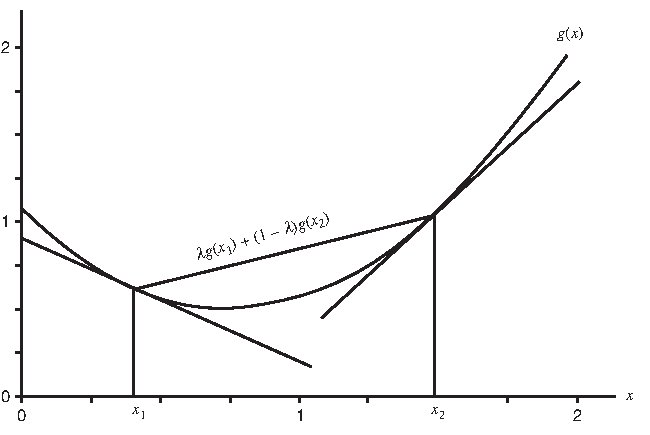
\includegraphics[width=.76\linewidth]{assets/chapter4/fig4-7-1.pdf}
\caption{凸函数及其在 $x_1$、$x_2$ 处的切线}\label{fig:4.7.1}
\end{figure}

\begin{definition}\label{def:4.7.6}\index{SI0121@凹函数}\index{SI0212@凸函数}
若对所有 $x,y$ 及 $0<\lambda<1$，都有 $g(\lambda x+(1-\lambda)y)\le\lambda g(x)+(1-\lambda)g(y)$，则称函数 $g(x)$ 为凸函数（convex function）. 若 $-g(x)$ 为凸函数，则称 $g(x)$ 为凹函数（concave function）.
\end{definition}
直观上，可以把凸函数看成“盛得住水”的函数，即形状像碗（例如 $g(x)=x^2$ 是凸的）；凹函数则会“把水洒出来”（例如 $g(x)=\log x$ 是凹的）. 更正式地说，凸函数位于连接图像上任意两点的直线下方，见\autoref{fig:4.7.1}. 当 $\lambda$ 从 0 变到 1 时，$\lambda g(x_1)+(1-\lambda)g(x_2)$ 描述连接 $g(x_1)$ 与 $g(x_2)$ 的线段. 若 $g(x)$ 为凸函数，此线段位于图像之上. 此外，凸函数位于其所有切线之上，\autoref{fig:4.7.1} 也显示了这一点；这正是 Jensen 不等式的基础.
\begin{theorem}[Jensen 不等式]\label{thm:4.7.7}\index{SI0569@Jensen}
对任意随机变量 $X$，若 $g(x)$ 为凸函数，则
$$Eg(X)\ge g(EX).$$
等号成立当且仅当对每条在 $x=EX$ 处与 $g(x)$ 相切的直线 $a+bx$，都有 $P(g(X)=a+bX)=1$.
\end{theorem}
\begin{proof}
为证明不等式，令 $l(x)$ 是 $g(x)$ 在 $g(EX)$ 处的切线. 回顾 $EX$ 是常数. 将其写为 $l(x)=a+bx$. \autoref{fig:4.7.2} 图示了这一情形.

由 $g$ 的凸性，$g(x)\ge a+bx$. 因为取期望保持不等式，有
$$\begin{aligned}
Eg(X)&\ge E(a+bX)\\
&=a+bEX&&\text{（期望的线性性，\autoref{thm:2.2.5}）}\\
&=l(EX)&&\text{（$l(x)$ 的定义）}\\
&=g(EX)&&\text{（$l$ 在 $EX$ 处相切）}
\end{aligned}$$
即所欲证.
\sourcepageanchor{187}

\begin{figure}[htbp]
\centering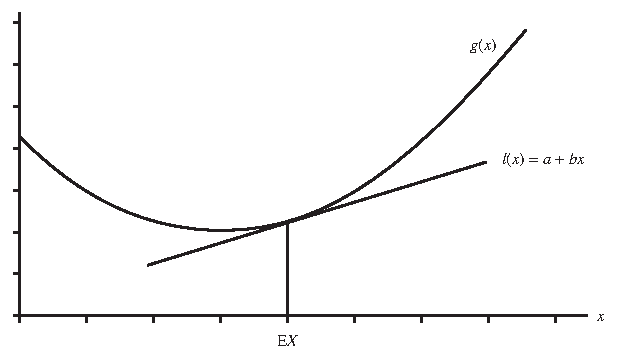
\includegraphics[width=.74\linewidth]{assets/chapter4/fig4-7-2.pdf}
\caption{Jensen 不等式的图示}\label{fig:4.7.2}
\end{figure}

如果 $g(x)$ 是线性的，则由期望的性质（\autoref{thm:2.2.5}）可知等号成立. 必要性部分见\autoref{exercise:4.62}.
\end{proof}
Jensen 不等式的一个直接应用是 $EX^2\ge(EX)^2$，因为 $g(x)=x^2$ 为凸函数. 又如，对正数 $x$，$1/x$ 为凸函数，因此 $E(1/X)\ge1/EX$，这也是一个有用的应用.

判断二次可微函数的凸性很容易：若对所有 $x$，$g''(x)\ge0$，则 $g(x)$ 为凸函数；若对所有 $x$，$g''(x)\le0$，则为凹函数. Jensen 不等式同样适用于凹函数：若 $g$ 凹，则 $Eg(X)\le g(EX)$.
\needspace{6\baselineskip}
\begin{example}[均值的不等式]\label{ex:4.7.8}\index{SI0064@算术平均数}\index{SI0457@几何平均数}\index{SI0468@调和平均数}\index{SI0573@均值}
Jensen 不等式可用于证明三种不同均值之间的不等式. 设 $a_1,\ldots,a_n$ 为正数，定义
$$\begin{aligned}
a_A&=\frac1n(a_1+a_2+\cdots+a_n),&&\text{（算术平均，arithmetic mean）}\\
a_G&=[a_1a_2\cdots a_n]^{1/n},&&\text{（几何平均，geometric mean）}\\
a_H&=\frac1{\frac1n\left(\frac1{a_1}+\frac1{a_2}+\cdots+\frac1{a_n}\right)}.&&\text{（调和平均，harmonic mean）}
\end{aligned}$$
它们之间满足
$$a_H\le a_G\le a_A.$$
为应用 Jensen 不等式，令 $X$ 的取值范围为 $a_1,\ldots,a_n$，且 $P(X=a_i)=1/n$，$i=1,\ldots,n$.\footnote{译注：若若干 $a_i$ 相同，严格说应在指标 $i\in\{1,\ldots,n\}$ 上均匀抽取，再令 $X=a_i$；重复取值的概率须合并. 原文逐值写 $P(X=a_i)=1/n$ 默认了取值不同，所给均值不等式对重复取值仍成立.} 因为 $\log x$ 为凹函数，Jensen 不等式给出 $E(\log X)\le\log(EX)$，所以
$$\begin{aligned}
\log a_G&=\frac1n\sum_{i=1}^n\log a_i=E(\log X)\le\log(EX)\\
&=\log\left(\frac1n\sum_{i=1}^na_i\right)=\log a_A,
\end{aligned}$$
故 $a_G\le a_A$. 再次利用 $\log x$ 的凹性，
$$\log\frac1{a_H}=\log\left(\frac1n\sum_{i=1}^n\frac1{a_i}\right)
=\log E\frac1X\ge E\left(\log\frac1X\right)=-E(\log X).$$
因为 $E(\log X)=\log a_G$，故 $\log(1/a_H)\ge\log(1/a_G)$，即 $a_G\ge a_H$.
\end{example}
\sourcepageanchor{188}

下一个不等式仅利用协方差的定义，但有时很有用. 如果随机变量 $X$ 有有限均值 $\mu$，且 $g(x)$ 为非减函数，则
$$E(g(X)(X-\mu))\ge0,$$
因为
$$\begin{aligned}
&E(g(X)(X-\mu))\\
&=E\bigl(g(X)(X-\mu)I_{(-\infty,0)}(X-\mu)\bigr)+E\bigl(g(X)(X-\mu)I_{[0,\infty)}(X-\mu)\bigr)\\
&\ge E\bigl(g(\mu)(X-\mu)I_{(-\infty,0)}(X-\mu)\bigr)\\
&\qquad+E\bigl(g(\mu)(X-\mu)I_{[0,\infty)}(X-\mu)\bigr)\qquad\text{（因为 $g$ 非减）}\\
&=g(\mu)E(X-\mu)\\
&=0.
\end{aligned}$$
推广这一论证，可以建立下面的不等式（见\autoref{exercise:4.65}）.
\begin{theorem}[协方差不等式]\label{thm:4.7.9}\index{SI0566@协方差}
设 $X$ 为任意随机变量，$g,h$ 为使 $Eg(X)$、$Eh(X)$ 和 $E(g(X)h(X))$ 均存在的函数.
\begin{enumerate}
\item[(a)]\phantomsection\label{itm:thm:4.7.9:a} 若 $g(x)$ 非减、$h(x)$ 非增，则
$$E(g(X)h(X))\le(Eg(X))(Eh(X)).$$
\item[(b)]\phantomsection\label{itm:thm:4.7.9:b} 若 $g(x),h(x)$ 同为非减函数或同为非增函数，则
$$E(g(X)h(X))\ge(Eg(X))(Eh(X)).$$
\end{enumerate}
\end{theorem}
不等式背后的直观很简单：\hyperref[itm:thm:4.7.9:a]{(a)} 中 $g$ 与 $h$ 负相关，\hyperref[itm:thm:4.7.9:b]{(b)} 中二者正相关；不等式只是反映了这一事实. 协方差不等式的用途在于，无须使用高阶矩，就可以给期望作界.
